% The LaTeX class file and the template have been created by Reimo Palm 
% with some modifications by the Institute of Computer Science of UT  
% following the guidelines of UT Press.
% 
% Last modified: 2025/03/26 v1.5
% See full list of authors in README.md
%
% Contact: ics@ut.ee

\documentclass{phdunitartu}
\usepackage{phdstyle}
\usepackage{assets/glossary}

%
\ThesisType{COLLECTION} % Possible values: MONOGRAPH, COLLECTION
%
\author{Firstname Lastname}
\title{Dissertation Title}

%
\institute{Institute of Computer Science} % Replace with your institute/college
\faculty{Faculty of Science and Technology} % Replace with your Faculty
\affiliation{University of Tartu}

%
\ISSN{1024-4212}           % will be provided by UT Press
\ISBNPRINT{978-9949-XX-XXX-X} % ISBN print, will be provided by UT Press
\ISBNPDF{978-9949-XX-XXX-X} % ISBN PDF, will be provided by UT Press

%
\dissertationseriesname{Dissertationes informaticae Universitatis Tartuensis}  % will be provided by UT Press
\dissertationseriesnumber{XX}  % will be provided by UT Press
\thesisfield{Computer Science} % Replace with your field
\commencementdate{XXX, 20XX} % Example: June, 2020
\defensedate{XX, 20XX} % Example: 01, 2020
\defensetime{XX:XX} % Example: 10:15
\defenseloc{XXX} % Example: Narva mnt 18-322

% supervisor(s)
\addSup{Supervisor}{
    Prof. & Firstname Lastname\\
    & Address\\
    & Address
}

% opponents
\addOpp{Opponents}{
    Prof. Dr.& Firstname Lastname\\
    &Address\\
    &Address\\
    &Address\\
    \\
    Prof. & Firstname Lastname\\
    &Address\\
    &Address
}

%
\addbibresource{bibliographies/publications.bib} % your publications
\addbibresource{bibliographies/bibliography.bib} % any other references
% why to use bibtex instead of manually listing the entries? check here: https://web.iit.edu/sites/web/files/departments/academic-affairs/graduate-academic-affairs/pdfs/biblio-help2.pdf

% to remove a chapter you can easily comment out from the following list
\includeonly
{
    extras/dedication,
    sections/0-1_abstract,
    extras/listofpublications,
    extras/abbreviations,
    sections/0-2_preface,
    sections/1_introduction,
    sections/2_background,
    sections/3-1_chapterI,
    sections/3-2_chapterII,
    sections/4_conclusion,
    sections/A_appendixA,
    sections/B_appendixB,
    extras/acknowledge,
    sections/summary_est,
    extras/publications,
    extras/cv_eng,
    extras/cv_est,
    extras/chapterpublications, % only for a monograph
}

\begin{document}
    \maketitle
    \thispagestyle{empty}
    \newpage\null\vskip35mm
\begin{flushright}
\itshape To my family and friends
\end{flushright}
    \setcounter{page}{6}
    \newpage\pagestyle{plain}

\chapter*{Abstract}

% generated by https://www.lipsum.com/
Lorem ipsum dolor sit amet, consectetur adipiscing elit. Mauris vulputate felis sit amet congue aliquam. Mauris semper nibh at odio ullamcorper feugiat nec vel enim. Cras fermentum pretium faucibus. Etiam sapien lectus, consequat sed sollicitudin at, hendrerit vel elit. Vivamus lacinia interdum iaculis. In lorem purus, ultrices ac hendrerit in, commodo in elit. Curabitur quis nisl facilisis, aliquam nibh nec, eleifend orci. Nunc vitae posuere ex, in imperdiet augue. Maecenas pellentesque, ligula et condimentum accumsan, lectus velit dictum eros, dapibus faucibus sapien ante vitae felis. Quisque non dui libero. Proin metus tortor, gravida ac massa id, bibendum lacinia orci. Suspendisse non dignissim mauris. Nulla at libero quam. Sed vitae varius risus, eget efficitur dolor. Nam consequat metus eget tortor placerat, id suscipit ligula vulputate.

Aliquam semper in leo vel viverra. Nunc fringilla felis quis magna auctor, quis pulvinar enim vestibulum. Cras nunc mi, volutpat in neque mattis, feugiat cursus dolor. Mauris varius bibendum erat, quis porta est suscipit a. Nulla facilisi. Aliquam non neque blandit, porttitor metus a, hendrerit urna. Etiam dignissim, justo rutrum molestie volutpat, turpis ipsum venenatis odio, sed pulvinar metus diam in tellus. Duis venenatis lectus nisi, gravida blandit eros imperdiet eget. Nam hendrerit quam dui, a consectetur dolor rhoncus nec. Vivamus et risus quis felis efficitur varius non non diam. Aliquam dapibus sit amet leo quis ullamcorper.

Aenean semper ligula eget dui sagittis, nec tincidunt ante ornare. Nam et arcu vestibulum justo fringilla consequat quis vitae urna. Cras eu mollis quam. Lorem ipsum dolor sit amet, consectetur adipiscing elit. Aenean fringilla nisi ac convallis iaculis. Nam nulla nulla, rutrum eget tempor id, aliquam quis dui. Suspendisse sed cursus leo. Praesent lacus lacus, venenatis eget consequat nec, malesuada placerat urna. Etiam et hendrerit eros. Cras eget cursus magna, in imperdiet dolor. Quisque efficitur pretium rhoncus.

    
    %
    \tableofcontents
    \listoffigures
    \listoftables
    \chapter*{List of abbreviations}

\renewcommand{\glossarysection}[2][]{\section*{#1}}
\printglossary[type=\acronymtype, ]
\printglossary[title=Nomenclature, ]

% change the glossaries from assets/glossary.sty and use gls{<glossary_entry>} to use it in the text. Check the example within the text!
    \IfThesisTypeIsCollection{\chapter*{List of original publications}
\addcontentsline{toc}{chapter}{List of original publications}

%
% Here are two options - use the same bibtex and formatting as stanard literature
% or alternatively write your own ready-formatted part highlighting contributions, etc... 
% 

% This part has a lot of freedom to highlight your publications and contributions
% Ctrl-/ (slash) to uncomment

% \begin{enumerate}[I]
    
%     \item First Author, \textbf{Second Athor}, and Thir Author.  The title of the publication. \textbf{Journal}, July 2016.     \\    
    
%     \textbf{Author contributions:} Performed the experiment; wrote the code and contributed to manuscript. 
%     \\

%     \item \textbf{Second Author} and Fourth Author. Second paper. \textbf{Journal Two}, August 2017.
    
%     \item First Author$^{*}$, \textbf{Second Author}$^{*}$, and Third Author. Title 3. \textbf{Scientific Reports}, November 2019. \\
%     $^{*}$ -- shared first author.
    

% \section*{Publications not included in the thesis}


%     \item First Author, \textbf{Second Athor}, and Thir Author.  Not in Thesis. \textbf{Journal also}, July 2016.

%     \item \textbf{Second Author} and Fourth Author. Fifth paper. \textbf{Journal Two}, August 2017.
    
%     \item First Author$^{*}$, \textbf{Second Author}$^{*}$, and Third Author. Title 3. \textbf{Scientific Reports}, November 2019. \\
%     $^{*}$ -- shared first author.
    
% \end{enumerate}

% \section*{Other published work of the author}

% More Latex friendly and concise way:

\nocite{*} % to make sure your publication is listed even if you do not cite it in the text!
\newrefcontext[sorting=none] % to keep the same order as you put in the publications.bib

% do not forget to tag your entries in publications.bib with the appropriate keyword so that it shows up under the correct title!
\section*{Publications included in the thesis}
\printbibliography[keyword={included},heading=none,env=roman-numerals]

\section*{Publications not included in the thesis}
\printbibliography[keyword={excluded},heading=none,env=roman-numerals,resetnumbers=false] 
% for reset numbering something you need to clear the cache to see it affecting the PDF output!
    
\section*{Other published work of the author}
\printbibliography[keyword={other}, heading=none,env=roman-numerals,resetnumbers=false]

\section*{Author’s contribution to the publications}

Lorem ipsum dolor sit amet, consectetur adipiscing elit. Aliquam sapien purus, sagittis sit amet fermentum sed, bibendum et purus. Nunc nec mattis ex, nec ornare risus. Sed ut euismod justo, sit amet lacinia diam. Donec dui sapien, congue id mi a, varius ultricies justo. In vestibulum nisi erat, quis iaculis sem commodo lacinia. Nullam in ante orci. Quisque magna dui, sollicitudin quis feugiat ut, condimentum quis tellus.}{}
    
    %
    \chapter*{Preface}\addcontentsline{toc}{chapter}{Preface}

% generated by https://www.lipsum.com/
Lorem ipsum dolor sit amet, consectetur adipiscing elit. Aenean nec diam turpis. Integer aliquam purus non mauris faucibus, in luctus ex tristique. Pellentesque consectetur metus neque, et malesuada diam gravida ac. Nullam eu facilisis metus, eget blandit justo. Praesent magna lorem, semper at ornare in, mattis lobortis nulla. Curabitur luctus faucibus diam, eu molestie tortor facilisis vitae. Nulla tempus iaculis quam nec dignissim. Mauris tincidunt gravida felis.

Nulla blandit nibh quis massa mollis, et ultrices leo posuere. Ut congue faucibus malesuada. Mauris non metus nec nunc porta egestas vitae vitae ex. Sed tincidunt malesuada massa a vehicula. Integer et elit eget erat viverra semper. Aenean hendrerit, odio quis sodales sollicitudin, turpis augue sagittis lacus, et tempor magna felis at nulla.

Aliquam luctus finibus congue. Suspendisse tristique sapien ac nulla porttitor pretium. Praesent viverra imperdiet sem quis sollicitudin. Integer in feugiat arcu. Sed eleifend non mauris quis eleifend. Morbi nec arcu at orci cursus convallis. Nullam ornare vestibulum commodo. Mauris mattis odio egestas ligula congue tincidunt. Phasellus interdum finibus lobortis. Vestibulum mollis varius nulla eu euismod.

Etiam non porttitor eros. Aenean nec sagittis sapien, non ultrices lorem. Vestibulum est turpis, blandit vitae aliquet id, hendrerit eget est. Class aptent taciti sociosqu ad litora torquent per conubia nostra, per inceptos himenaeos. Duis ut ultricies elit. Pellentesque vitae blandit urna. Fusce sollicitudin, leo sed egestas ornare, eros ipsum suscipit lacus, sed faucibus turpis nisi vitae felis. Curabitur vel hendrerit mauris. Cras blandit purus elit, sit amet convallis eros scelerisque vitae. Suspendisse justo orci, placerat in metus sit amet, faucibus pharetra augue. Nam ut tellus at mauris iaculis maximus. Pellentesque ac est eu lorem volutpat tincidunt ac vitae diam. In aliquam diam non quam eleifend suscipit. Praesent lobortis dui et leo rutrum, sit amet scelerisque risus iaculis. Mauris mattis sollicitudin lectus, tristique bibendum neque viverra eget. Vivamus nec sem eget ex fringilla egestas eu et justo.
    
    \chapter{Introduction}

This template is designed to format doctoral theses by PhD students at the Institute of Computer Science. It contains the main structure and functionality that is required for writing the thesis.

The University of Tartu Press general guidelines\footnote{\url{https://tyk.ee/et/nouded-kasikirjadele}, December 3, 2024} have been followed in the template. Additional requirements for the thesis can be found in the Regulations for Doctoral Studies and Study Regulations\footnote{\url{https://sisu.ut.ee/ope/requirements-doctoral-thesis/?lang=en}}.

The template is split into multiple files and folders:

\begin{itemize}
\item \texttt{phdunitartu.cls}: A class file for both monograph and collection of publications type of theses;
\item \texttt{phdstyle.sty}: A style file for both monograph and collection of publications type of theses;
\item \texttt{main.tex}: The main file for the template with the thesis details need to be filled here;
\item \texttt{assets/glossary.sty}: a file containing all glossary entries.
\item \texttt{bibliographies/bibliography.bib}: A bibliography file for cited works
\item \texttt{bibliographies/publications.bib}: A bibliography file for author's publications
\item \texttt{sections/}: directory to keep the main content of thesis in, children files reflect the main document structure
\item \texttt{extras/}: other chapters required in the thesis
\item \texttt{assets/figures/}: to store the figures for the document
\item \texttt{assets/publications/}: a directory to store the PDF files of the publications to be included
\item \texttt{assets/tables/}: a directory to store the tables
\item \texttt{README.md}: a readme file documenting how the template is maintained.
\end{itemize}

The template contains two sample content chapters. Chapter \ref{chapterI} contains information about permitted changes to the template and a list of things that the author is not allowed to change. Chapter \ref{chapterII} provides examples of using the glossary, references, including figures and tables, and other commands in the template.
    
    \chapter{Background}

...

    % body
    \chapter{Content chapter I}
\label{chapterI}

This sample content chapter includes information about permitted changes and a list of things the author is not allowed to change. The information below is not exhaustive, therefore, please familiarize yourself with the UT doctoral thesis requirements\footnote{\url{https://sisu.ut.ee/ope/requirements-doctoral-thesis/?lang=en}}. In case these requirements conflict with the information in this template, the UT requirements should be followed.

\section{Things that should not be changed}

You should \textbf{not} change:

\begin{itemize}
    \item The text area size, as well as horizontal and vertical margins;
    \item The main font size and font itself;
    \item Font sizes and fonts of the titles.
\end{itemize}

Most of the sections (introduction, bibliography, conclusion, summary in Estonian) included are mandatory according to the UT regulations and may not be removed.

Sections \textit{Curriculum Vitae}, \textit{Elulookirjeluds} (CV in Estonian) and \textit{List of original publications} belong to the format of \textit{Dissertationes informaticae Universitatis Tartuensis} series and should not be omitted.

In a dissertation of the collection type, the section \textit{Publications included in the thesis} should list all papers whose reprints are included in the thesis and no others. Other original publications may be listed in separate sections. In case of listing publications with several authors, the author's contribution has to be described in the section \textit{Author’s contribution to the publications}.

Every reprinted publication in section \textit{Publications} should be preceded by a separate page containing its full publication record.

\section{Tolerable changes}

UT Press prefers to get the dissertation PDF files with a4 paper size. This means that the text area is much smaller than the page. The page will be cut to the right size by the UT Press. During writing, however, you may obtain a more adequate appearance of the result if you replace \texttt{a4paper} with \texttt{b5paper} in the class file. This change does not harm any other measures.

The order of sections in the template follows a standard thesis structure and should not be changed in most cases. Please modify it with responsibility and care. Note that the sections and their order are slightly different in monograph and collection types of the thesis. This is intentional. Please make sure to use the right template by calling the \texttt{ThesisType} command with the right value when you start writing.

Numbering of chapters is also intended to remain unchanged. So, an abstract, list of contents, list of figures, tables and abbreviations, bibliography, acknowledgement, summary in Estonian, publications, and CV should not be numbered, while the introduction and conclusion should preferably be numbered. The principle behind this choice is that both the introduction and conclusion are parts of the thesis. If you find this principle not being true, you may omit numbers of the introduction and conclusion, too. The recommended style of numbering uses arabic numbers in the main part and Latin alphabet for appendices. You are free to change it if you prefer.

Y\textbf{ou are expected to change} the values of “Dissertation title”, content chapter and (sub)section titles, appendix titles, “Töö pealkiri” (the thesis title in Estonian in the Estonian summary chapter). Please do not substitute other chapter names, for instance, "Sisukokkuvõte" (Summary in Estonian). Substituting, “Introduction” and “Conclusion” by something more precise is tolerable under good reasons.

Abstract, list of figures, list of tables, list of abbreviations, preface and acknowledgement may be omitted. In a dissertation of the collection type, not all subsections of “List of original oublications” given in the example are mandatory. If you only list publications whose reprints are included in the thesis, please remove the subsection and rename the section title to “Publications included in the thesis”.

The student may use any reference style out of the three standard ones. Likewise, choice of the format of the bibliographic records in the bibliography section, list of publications, and before each reprinted publication (in a thesis of the collection type) is up to the author of the thesis. The same style must be used throughout the thesis.

In a thesis of the collection type, it is recommended to include each publication also in the general list of contents of the thesis, as shown in the example. Alternately, a separate list of contents for the reprinted publications may be created.
    \chapter{Content chapter II}
\label{chapterII}

This sample content chapter includes examples of using the template.

\section{Citing}

This is an example of citing your own papers \parencite{paper1,paper2} in addition to just listing them under publications and making them show up in the bibliography. You can reference other papers \parencite{einstein, knuthwebsite,latexcompanion} like this.

Three different citation styles (\texttt{authoryear}, \texttt{numeric}, \texttt{alphabetic}) have been enabled in the template. To select your peferred citation style, uncomment the corresponding \texttt{style=...} line in the "Bibliography" section in \texttt{phdstyle.sty}.

While the template uses \texttt{biblatex}\footnote{\url{https://www.overleaf.com/learn/latex/Bibliography_management_with_bibtex}} to manage bibliography and citations, compatibility mode with \texttt{natbib} has been enabled. Therefore, you can use \texttt{biblatex} commands such as \texttt{\textbackslash parencite} or \texttt{\textbackslash textcite}, or their respective \texttt{natbib} equivalents \texttt{\textbackslash citep} or \texttt{\textbackslash citet}. If you experience any issues with the \texttt{natbib} commands, \texttt{biblatex} commands may be more stable.

In case of \texttt{numeric} and \texttt{alphabetic} styles, \texttt{\textbackslash cite}, \texttt{\textbackslash parencite} (or \texttt{\textbackslash citep}) are equivalent and will just show the citation in square brackets. The three commands differ, however, for the \texttt{authoryear} style:

\begin{itemize}
    \item \texttt{\textbackslash cite} will mention the author and year without using any parenthesis: \cite{einstein}
    \item \texttt{\textbackslash parencite} or \texttt{\textbackslash citep} will put the entire citation into parenthesis: \parencite{einstein}
    \item \texttt{\textbackslash textcite} or \texttt{\textbackslash citet} will mention the author in text and put the year into parenthesis (or the number or alphabetic reference into square brackets when using other citation styles): \textcite{einstein}
\end{itemize}

\section{Using the glossary}
If you wish to include a glossary, you can define items in \texttt{glossary.sty}.

You can use the defined acronyms with the \texttt{\textbackslash gls} command like this: \gls{ut}, \gls{ny}, \gls{la}, \gls{un}. This will print the acronym and its definition the first time and just the acronym all following times like this: \gls{ut}. To manually set whether only the acronym, only the definiton or both should be printed, commands \texttt{\textbackslash acrshort}, \texttt{\textbackslash acrlong} and \texttt{\textbackslash acrfull} can be used.

The nomenclature items can also be used with the \texttt{\textbackslash gls} command like this: \gls{angelsperarea}, \gls{numofangels}, \gls{areaofneedle}. For more information about using the glossary, check out the documentation\footnote{\url{https://www.overleaf.com/learn/latex/Glossaries}}.

\section{Inserting figures and tables}

% generated by https://www.lipsum.com/
Lorem ipsum dolor sit amet, consectetur adipiscing elit. Aenean nec diam turpis. Integer aliquam purus non mauris faucibus, in luctus ex tristique. Pellentesque consectetur metus neque, et malesuada diam gravida ac. Nullam eu facilisis metus, eget blandit justo. Praesent magna lorem, semper at ornare in, mattis lobortis nulla. Curabitur luctus faucibus diam, eu molestie tortor facilisis vitae. Nulla tempus iaculis quam nec dignissim. Mauris tincidunt gravida Fig.~\ref{fig:my_label} felis.

\begin{figure}[htp]
    \centering
    
\includegraphics[width=7cm]{assets/figures/overleaf_wide_colour_green_bg.png}
    \caption{A sample figure}
    \label{fig:my_label}
\end{figure}

Vestibulum est turpis, blandit vitae aliquet id, hendrerit eget est. Class aptent taciti sociosqu ad litora torquent per conubia nostra, per inceptos himenaeos. Duis ut ultricies elit. Pellentesque vitae blandit urna. Fusce sollicitudin, leo sed egestas ornare, eros ipsum suscipit lacus, sed faucibus turpis nisi vitae felis. Curabitur vel hendrerit mauris. Cras blandit purus elit, sit amet convallis eros Table~\ref{tab:my_label} scelerisque.

\begin{table}[h]
    \centering
    \caption{A sample table}
    \label{tab:my_label}
    \begin{tabular}{||c| c c c||}
        \hline
        Col1 & Col2 & Col2 & Col3 \\ [0.5ex]
        \hline\hline
        1 & 6 & 87837 & 787 \\
        \hline
        2 & 7 & 78 & 5415 \\
        \hline
        3 & 545 & 778 & 7507 \\
        \hline
        4 & 545 & 18744 & 7560 \\
        \hline
        5 & 88 & 788 & 6344 \\ [1ex]
        \hline
    \end{tabular}
\end{table}

Nam feugiat, nisl vel consectetur tempus, metus eros gravida orci, a semper odio odio sed erat. Donec in metus orci. Proin ultrices condimentum ligula, et posuere tortor ultricies vel. Sed dictum id tellus in consectetur. Donec scelerisque ullamcorper eros at hendrerit. Vivamus varius laoreet felis, non congue enim blandit ac. Vivamus maximus dolor eget mauris faucibus, a tempus mi facilisis. Integer mollis blandit dolor nec varius.

    % conclusion
    \chapter{Conclusion}

Lorem ipsum dolor sit amet, consectetur adipiscing elit. Duis mattis vehicula neque nec feugiat. Sed sem nunc, vehicula eu vulputate quis, faucibus nec nunc. Nulla in augue turpis. Suspendisse at auctor tortor. Duis scelerisque felis ac libero condimentum, congue aliquam enim commodo. Integer in nisi ornare, rhoncus nisi dapibus, gravida nunc. Quisque tincidunt ac justo ac aliquet. Maecenas vulputate consequat metus. Nullam faucibus fringilla purus.

Phasellus tempus felis in lectus pretium volutpat. Vivamus in nisi diam. Mauris laoreet semper bibendum. Aliquam fringilla ut purus rutrum porta. Duis laoreet pretium felis, a malesuada justo lacinia sed. Duis sem justo, interdum eget purus eget, interdum aliquam leo. Donec molestie, dolor nec dapibus lacinia, ipsum justo convallis felis, nec elementum mi diam nec neque. Aliquam venenatis ex non sapien convallis ullamcorper. Mauris congue rutrum finibus. Nam hendrerit venenatis ultrices. Ut non libero tellus. Nulla sollicitudin, justo non mollis maximus, dui dolor porta erat, nec laoreet turpis eros non nibh. Vestibulum sed mauris laoreet, condimentum enim sed, fermentum eros. Vivamus congue nibh dictum rhoncus euismod.

    % bibliography
    % you can change the bibliography style from the phdstyle.sty file, bibliography section
    % \nocite{*} % by adding this line, also references not cited in text will be shown in the biblography list. This can be useful while editing, but shouldn't be used in the final version.
    \printbibliography

    %
    \appendix
    \chapter{Appendix title}
\section{Appendix section title}
\section{Appendix section title}

    \chapter{Appendix title}

    %
    \setcounter{secnumdepth}{-1}
    \chapter{Acknowledgements}

% generated by https://www.lipsum.com/
Lorem ipsum dolor sit amet, consectetur adipiscing elit. Aenean nec diam turpis. Integer aliquam purus non mauris faucibus, in luctus ex tristique. Pellentesque consectetur metus neque, et malesuada diam gravida ac. Nullam eu facilisis metus, eget blandit justo. Praesent magna lorem, semper at ornare in, mattis lobortis nulla. Curabitur luctus faucibus diam, eu molestie tortor facilisis vitae. Nulla tempus iaculis quam nec dignissim. Mauris tincidunt gravida felis. 
    \begin{otherlanguage}{estonian}
\chapter*{Sisukokkuv\~ote}
\addcontentsline{toc}{chapter}{Sisukokkuv\~ote (Summary in Estonian)}

\section*{T\"o\"o pealkiri} % Thesis title in Estonian

\end{otherlanguage} % summary in Estonian
    \IfThesisTypeIsCollection{\ifodd\value{page}\else\newpage\null\thispagestyle{empty}\fi

\chapter{Publications}
\thispagestyle{empty}


\newpage\null\thispagestyle{empty}

% Publication I

\ifodd\value{page}\else\newpage\thispagestyle{empty}\fi
\marginpar{

\begin{tikzpicture}
      \draw[fill,color=black] (0,0) rectangle (4cm,2cm);
      \draw[color=white] (1cm,1cm) node {\normalfont\huge\bfseries I};
\end{tikzpicture}
}
\newpage

\phantomsection\addcontentsline{toc}{section}{First article title}
\thispagestyle{empty}\null\vfill
\begin{flushright}
F. Author, S. Author\\
First article title\\
Journal, number, pages\\
\medskip
The article is reprinted with permission of the copyright owner.
\end{flushright}

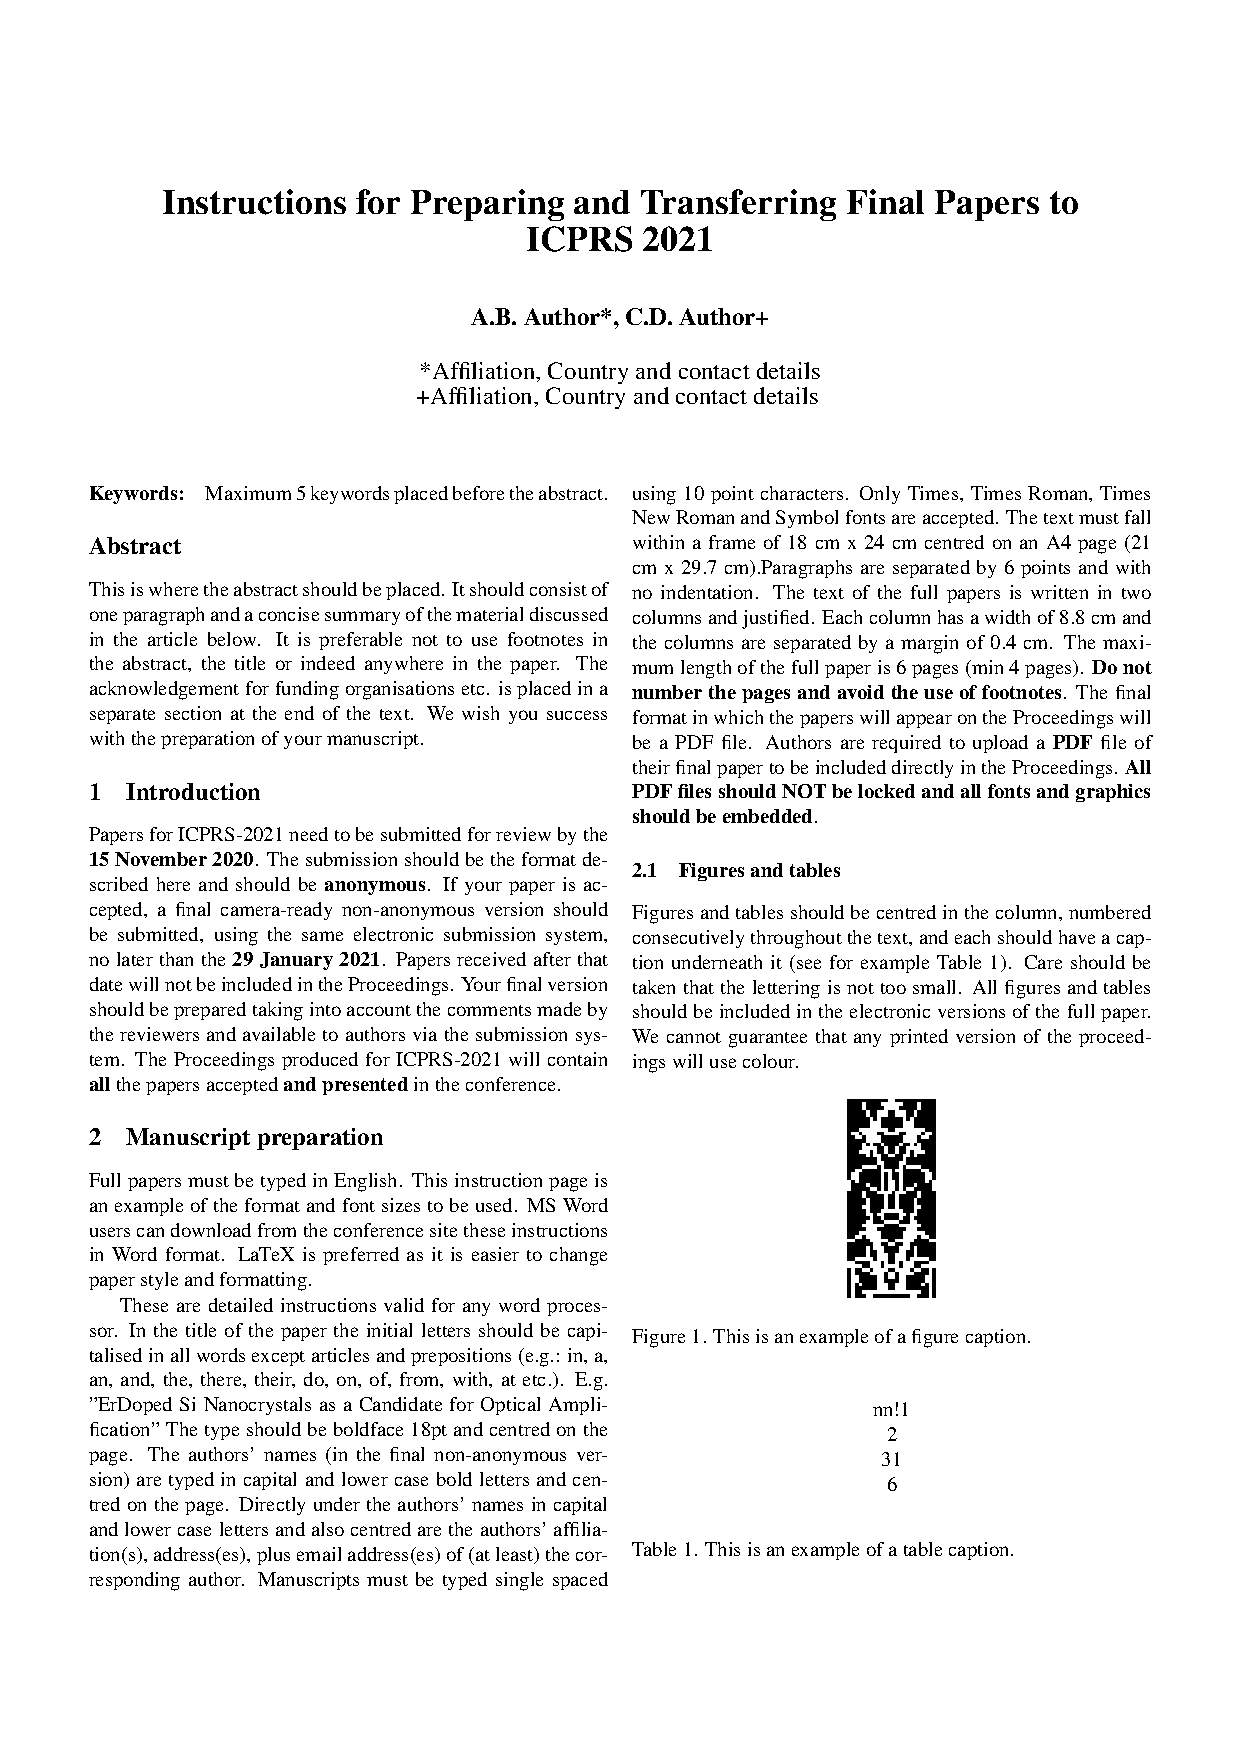
\includepdf[pages=-]{assets/publications/icprs-template-article.pdf}

\newpage\null\thispagestyle{empty}

% Publication II

\ifodd\value{page}\else\newpage\thispagestyle{empty}\fi
\marginpar{

\begin{tikzpicture}
      \draw[fill,color=black] (0,0) rectangle (4cm,2cm);
      \draw[color=white] (1cm,1cm) node {\normalfont\huge\bfseries II};
\end{tikzpicture}
}
\newpage

\phantomsection\addcontentsline{toc}{section}{Second article title}
\thispagestyle{empty}\null\vfill
\begin{flushright}
F. Author, S. Author\\
Second article title\\
Journal, number, pages\\
\medskip
The article is reprinted with permission of the copyright owner.
\end{flushright}

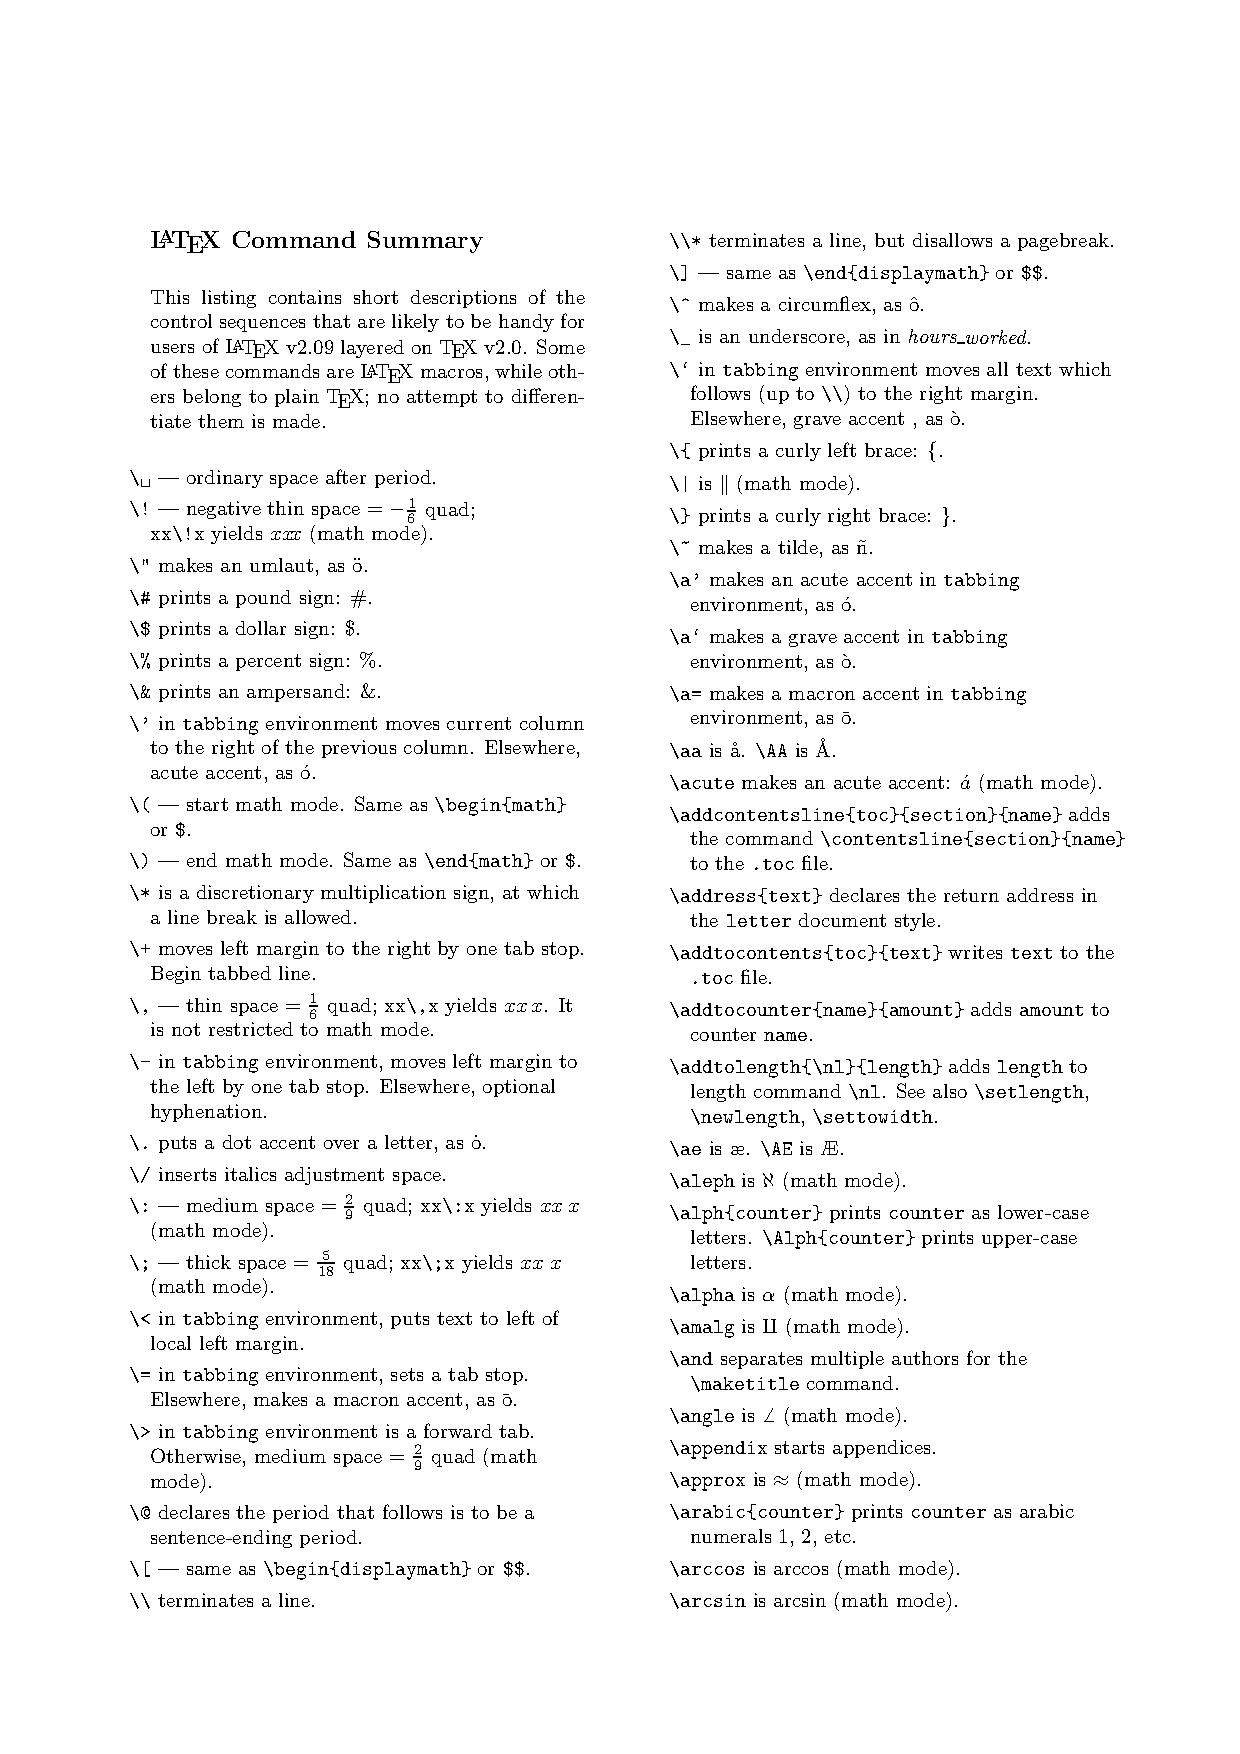
\includepdf[pages=-]{assets/publications/ltxcrib.pdf}

\newpage\null\thispagestyle{empty}}{}

    % curriculum vitae
    \chapter{Curriculum Vitae}

\section*{Personal data}

\begin{tabular}{@{}l@{\hskip7mm}l}
XXX:       &XXX\\
XXX:       &XXX\\
XXX:       &XXX\\
XXX:       &XXX
\end{tabular}

\section*{Education}

\begin{tabular}{@{}l@{\hskip7mm}p{90mm}}
XXXX--XXXX         & XXX\\
XXXX--XXXX         & XXX\\
XXXX--XXXX         & XXX
\end{tabular}

\section*{Employment}

\begin{tabular}{@{}l@{\hskip7mm}p{90mm}}
XXXX--XXXX         & XXX\\
XXXX--XXXX         & XXX\\
XXXX--XXXX         & XXX
\end{tabular}

\section*{Scientific work}

Main fields of interest:
\begin{itemize}
  \item XXX
  \item XXX
  \item XXX
\end{itemize} % English
    \begin{otherlanguage}{estonian}
\chapter*{Elulookirjeldus}
\addcontentsline{toc}{chapter}{Elulookirjeldus (Curriculum Vitae in Estonian)}

\section*{Isikuandmed}

\begin{tabular}{@{}l@{\hskip7mm}l}
XXX:       &XXX\\
XXX:       &XXX\\
XXX:       &XXX\\
XXX:       &XXX
\end{tabular}

\section*{Haridus}

\begin{tabular}{@{}l@{\hskip7mm}p{90mm}}
XXXX--XXXX         & XXX\\
XXXX--XXXX         & XXX\\
XXXX--XXXX         & XXX
\end{tabular}

\section*{Teenistusk\"aik}

\begin{tabular}{@{}l@{\hskip7mm}p{90mm}}
XXXX--XXXX         & XXX\\
XXXX--XXXX         & XXX\\
XXXX--XXXX         & XXX
\end{tabular}

\section*{Teadustegevus}

Peamised uurimisvaldkonnad:
\begin{itemize}
  \item XXX
  \item XXX
  \item XXX
\end{itemize}
\end{otherlanguage}
 % Estonian
    \IfThesisTypeIsCollection{}{% This chapter is used in a monograph
\chapter{List of original publications}
}
\end{document}